\documentclass[11pt,letter, swedish, english
]{article}
\pdfoutput=1

\usepackage{../custom_as}

\usepackage{listings} 
\usepackage[framed,numbered,autolinebreaks,useliterate]{../mcode}
\lstloadlanguages{matlab} 
\lstset{language=matlab} 

\usepackage[makeroom]{cancel}
\graphicspath{{figures/}}


\swapcommands{\Omega}{\varOmega}

%%Drar in tabell och figurtexter
\usepackage[margin=10 pt]{caption}
%%För att lägga in 'att göra'-noteringar i texten
\usepackage{todonotes} %\todo{...}

%%För att själv bestämma marginalerna. 
\usepackage{geometry}

%%För att ändra hur rubrikerna ska formateras


%\renewcommand{\thefootnote}{\fnsymbol{footnote}}

\renewcommand{\thesubsection}{\arabic{section} (\alph{subsection})}
\renewcommand{\thesubsubsection}{\arabic{section} (\alph{subsection},\,\roman{subsubsection})}

\newcommand{\Dx}{\ensuremath{\Delta{x}}}
\newcommand{\Dt}{\ensuremath{\Delta{t}}}

\begin{document}




%%%%%%%%%%%%%%%%% vvv Inbyggd titelsida vvv %%%%%%%%%%%%%%%%%

\title{Numerical solutions to PDE's -- AMATH\,741 \\
Assignment 3}
\author{Andréas Sundström}
\date{\today}

\maketitle

%%%%%%%%%%%%%%%%% ^^^ Inbyggd titelsida ^^^ %%%%%%%%%%%%%%%%%

\section{Numerical investigation of numerical dissipation and dispersion}
In this problem we will be deal ing with numerical schemes of the form
\begin{equation}
U_j^{n+1}=(1-\beta)U_j^n+\frac{\beta-\alpha}{2}U_{j+1}^n+\frac{\alpha+\beta}{2}U_{j-1}^n
\end{equation}
for solving the linear advection equation $u_t+au_x=0$. Here
$\alpha=a\Dt/\Dx$ and $\beta$ depends on the scheme:
\begin{center}
\begin{tabular}{l|c|c|c|c|}\cline{2-5}
&Upwind&Lax-Friedrichs&Lax-Wendroff&Centered\\ \hline
\multicolumn{1}{|l|}{$\beta$: }&$|\alpha|$&$1$&$\alpha^2$&0\\ \hline
\end{tabular}
\end{center}

It is easy to show that, with \emph{periodic boundary conditions},
each time step can be represented using a transfer matrix,
$U^{n+1}=\mathsf{T}U^n$ where
\begin{equation}
T=\begin{bmatrix}
D_0&D_{+1}&0&\cdots&0&0&D_{-1}\\
D_{-1}&D_0&D_{+1}&0&\cdots&0&0\\
0&D_{-1}&D_0&D_{+1}&0&\cdots&0\\
\vdots&&&\ddots&&&\vdots\\
0&\cdots&0&D_{-1}&D_0&D_{+1}&0\\
0&0&\cdots&0&D_{-1}&D_0&D_{+1}\\
D_{+1}&0&0&\cdots&0&D_{-1}&D_0\\
\end{bmatrix}
\end{equation}
and $D_0=(1-\beta)$, $D_{-1}=(\alpha+\beta)/2$ and
$D_{+1}=(\beta-\alpha)/2$. 
This is them implemented in MATLAB through:
\lstinputlisting{code/spTranferMatrix.m}
With the matrix, the rest is just a matter of looping through all time
steps.  

\subsection{Numerical dissipation depending on $\Dx$}
\begin{figure}
\centering
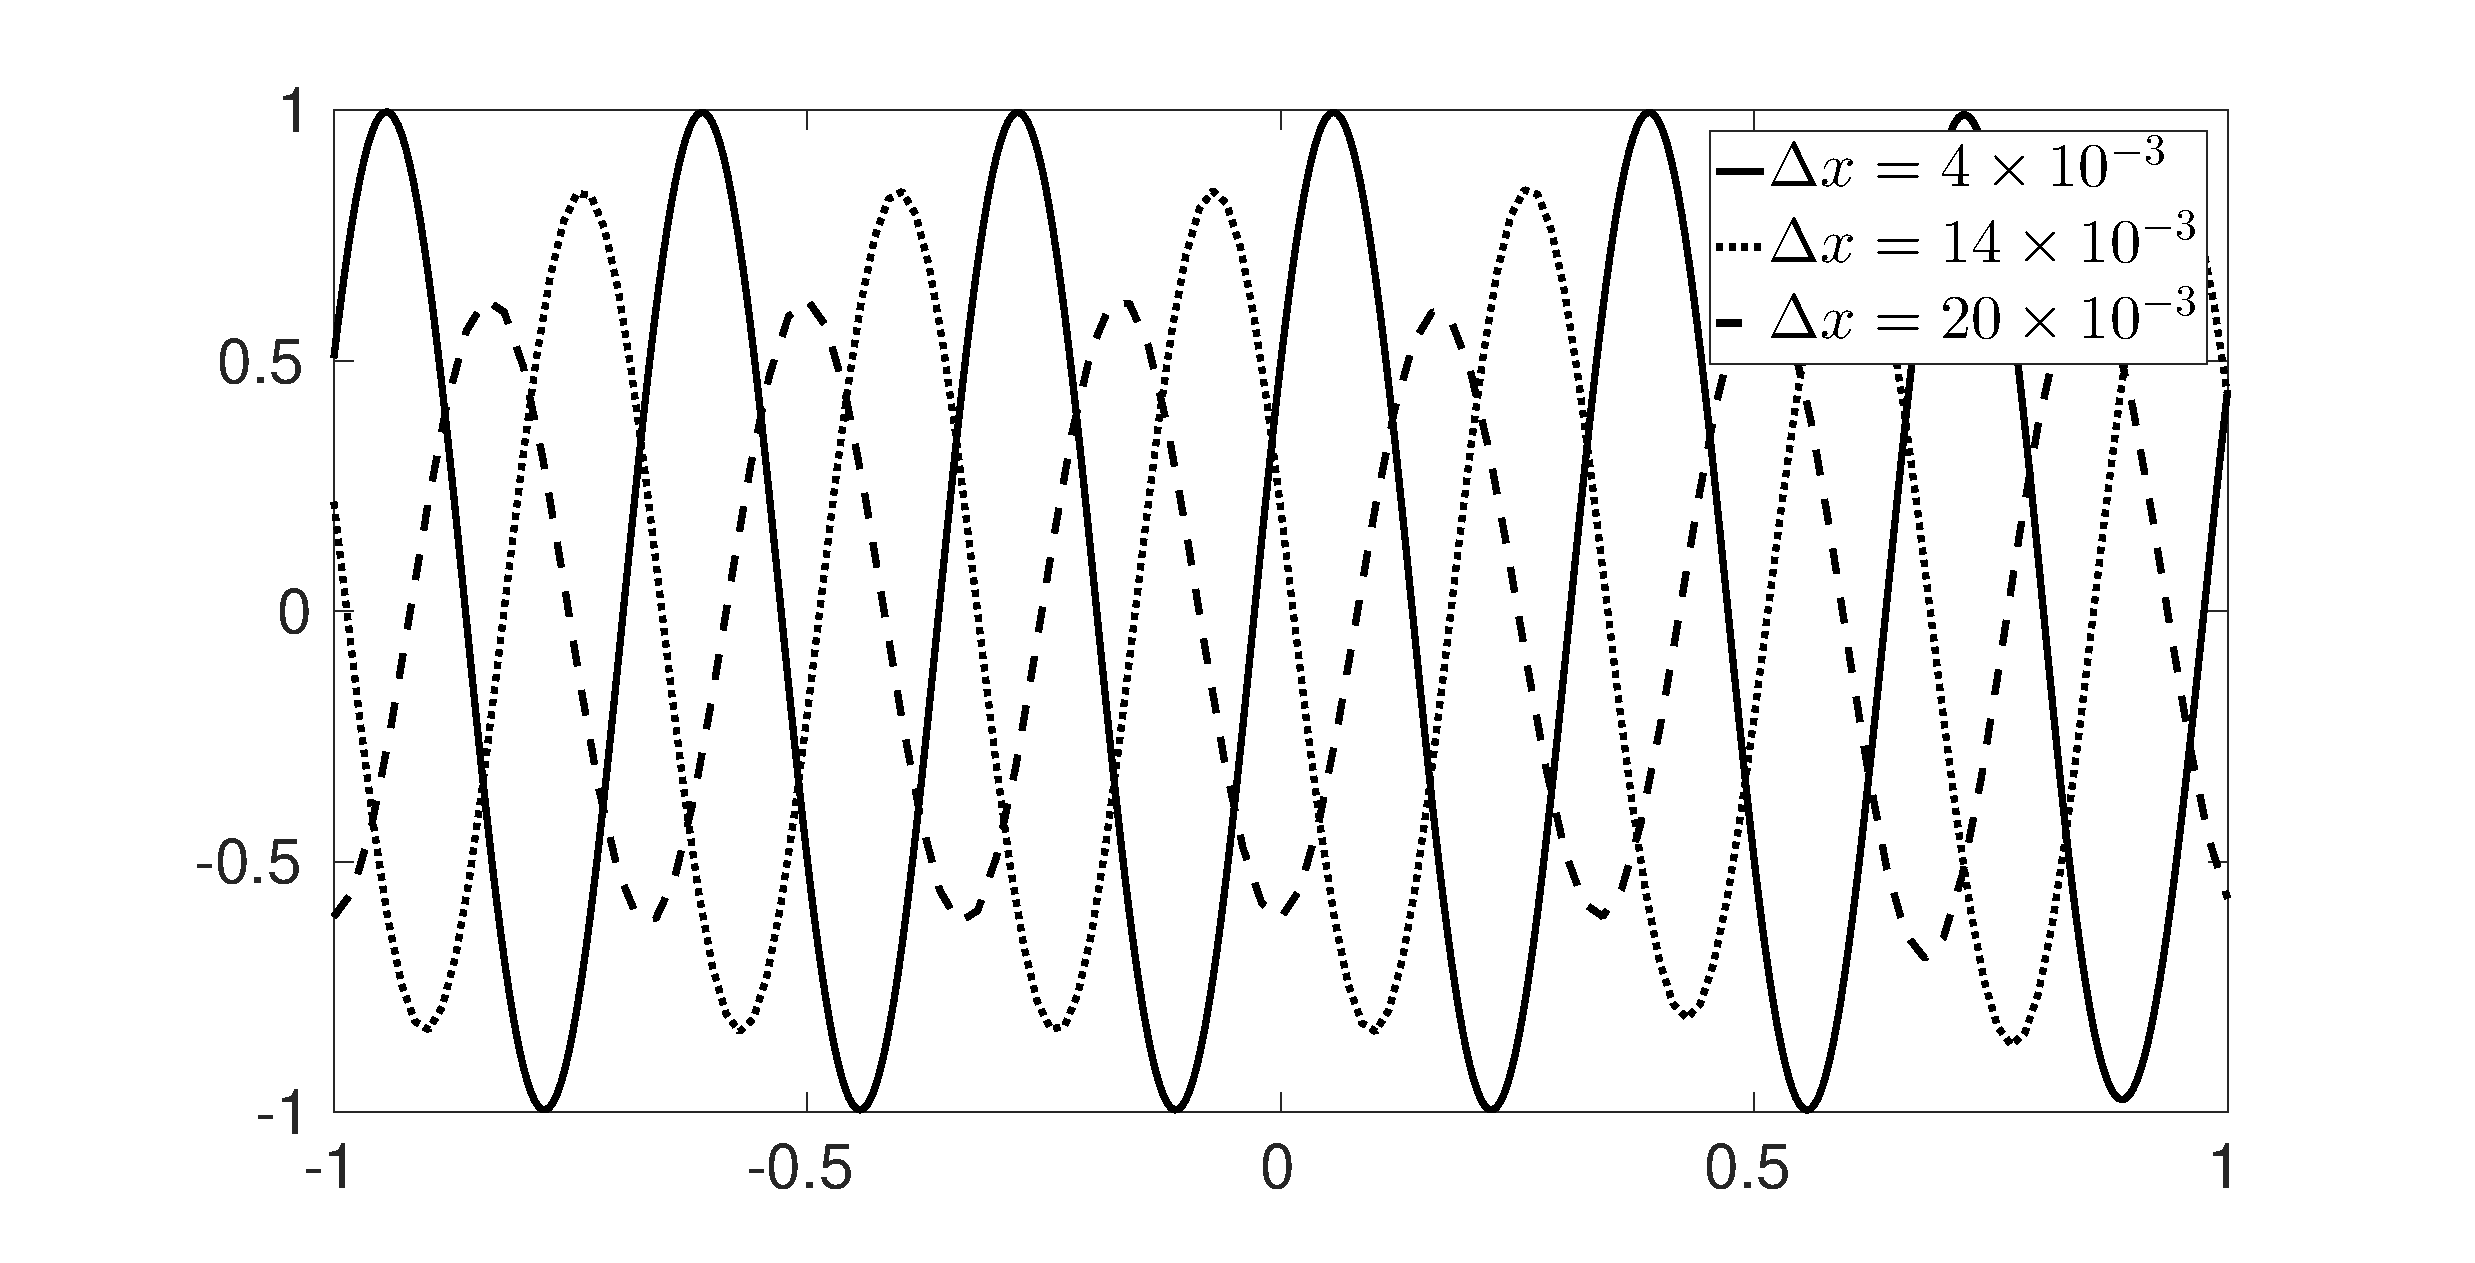
\includegraphics[width=1\textwidth]{1a.eps}
\caption{}
\label{fig:1a}
\end{figure}

\subsection{Numerical dissipation depending on scheme}
\begin{figure}
\centering
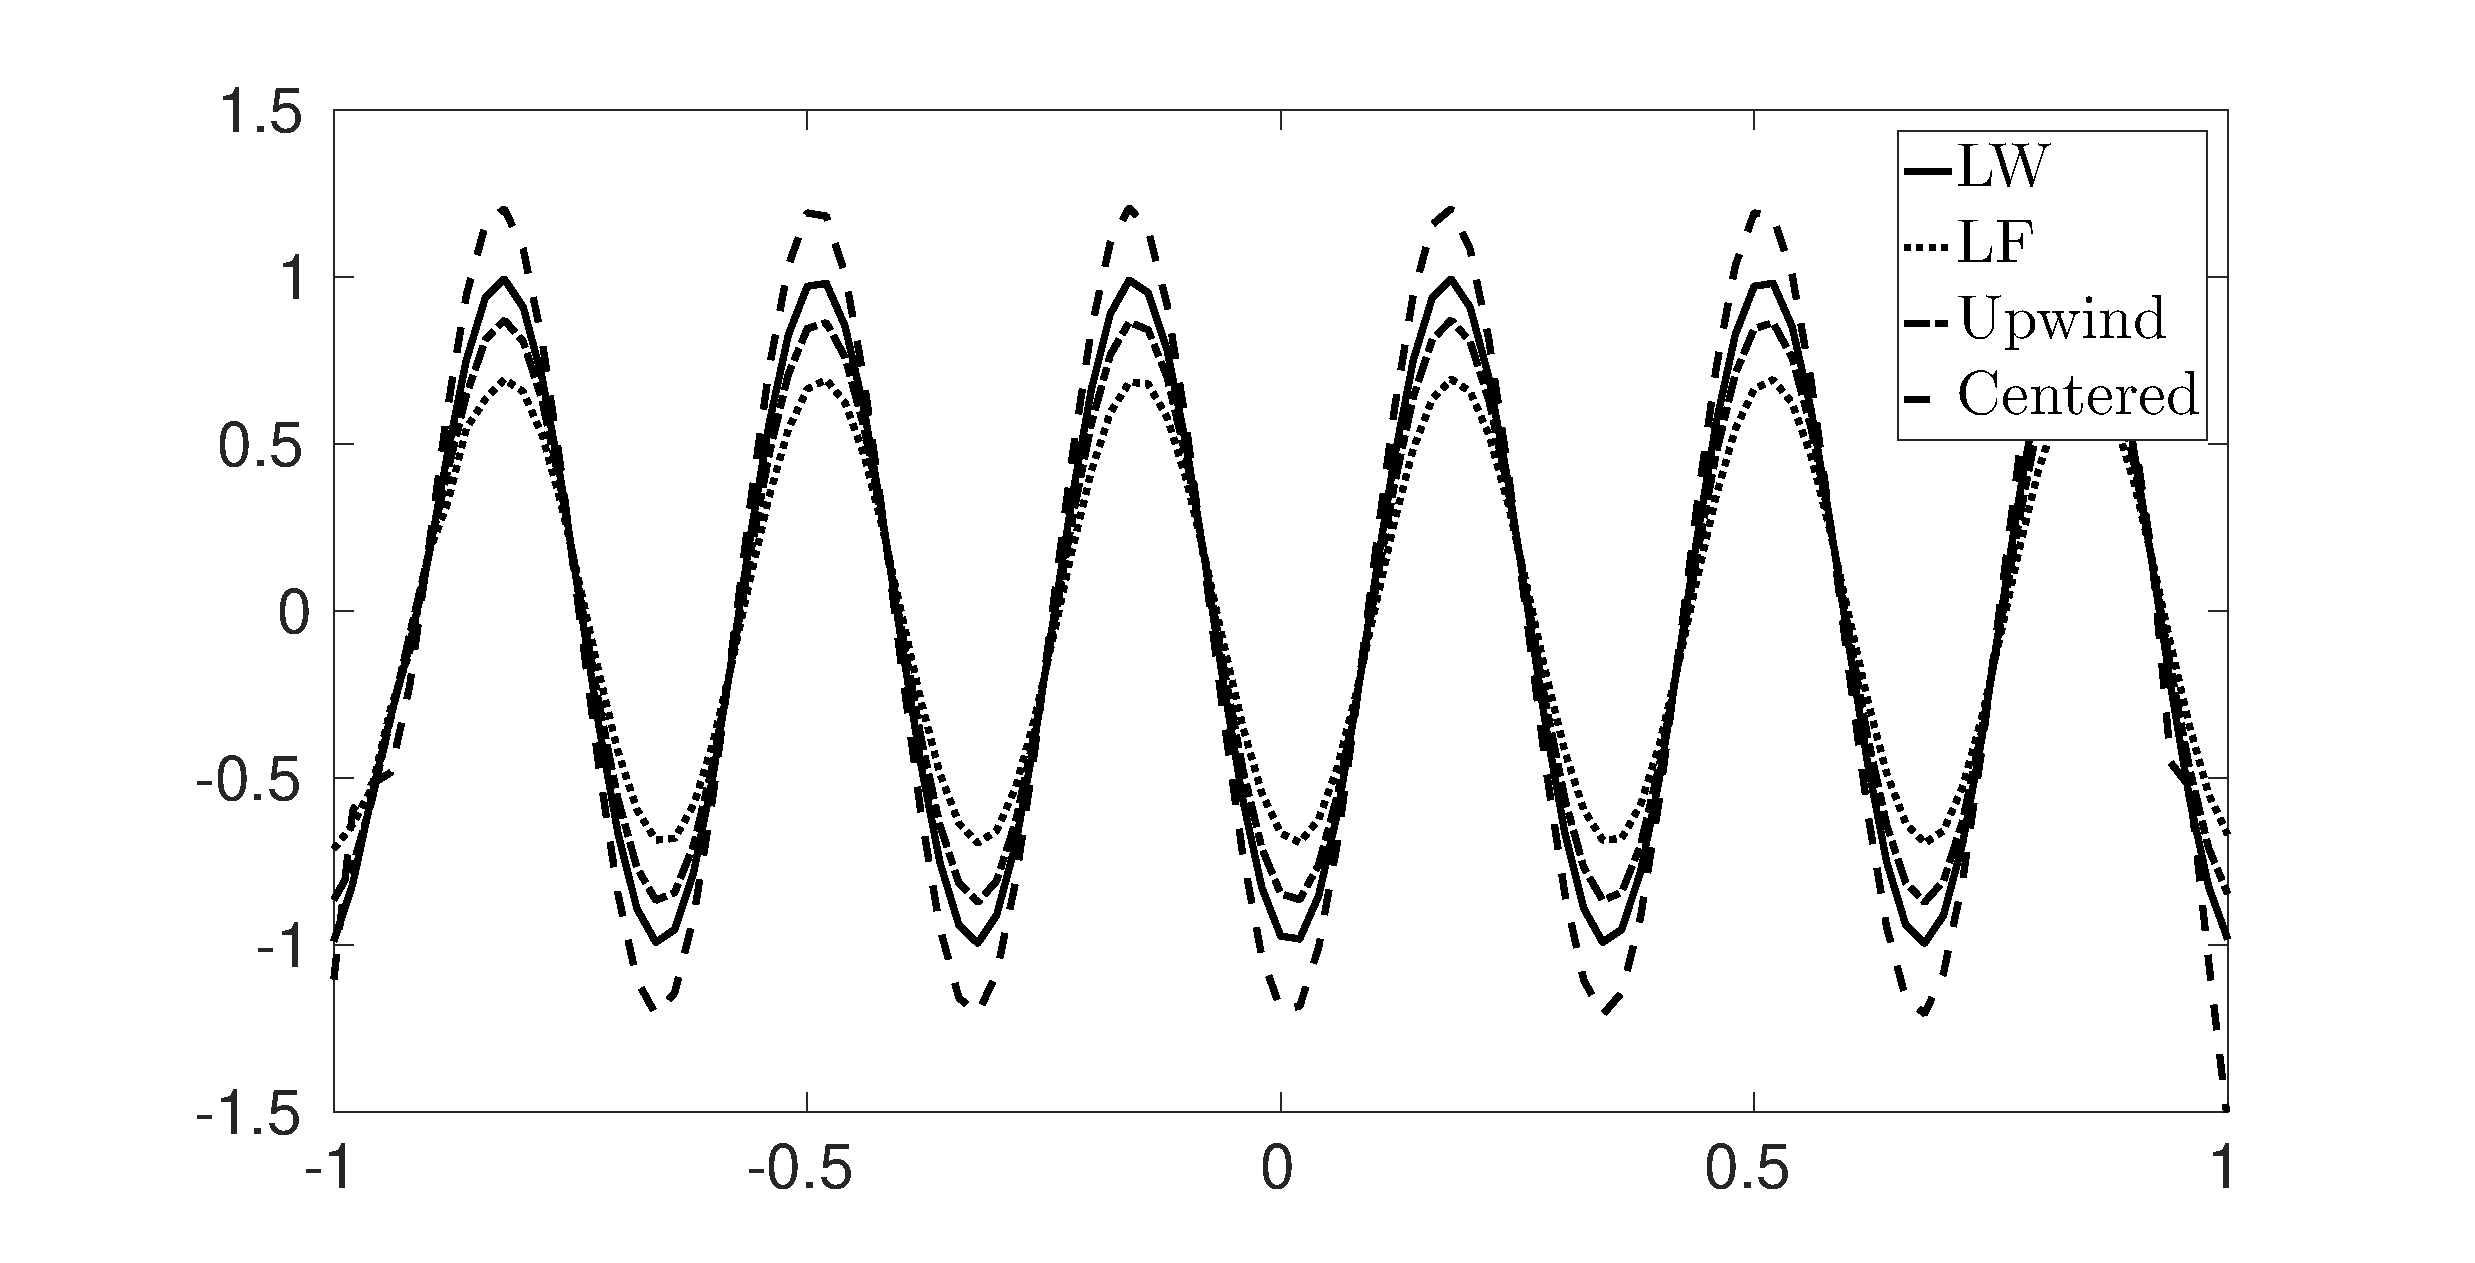
\includegraphics[width=1\textwidth]{1b.eps}
\caption{}
\label{fig:1b}
\end{figure}


\subsection{The affects of the size of $\Dt$}
\begin{figure}
\centering
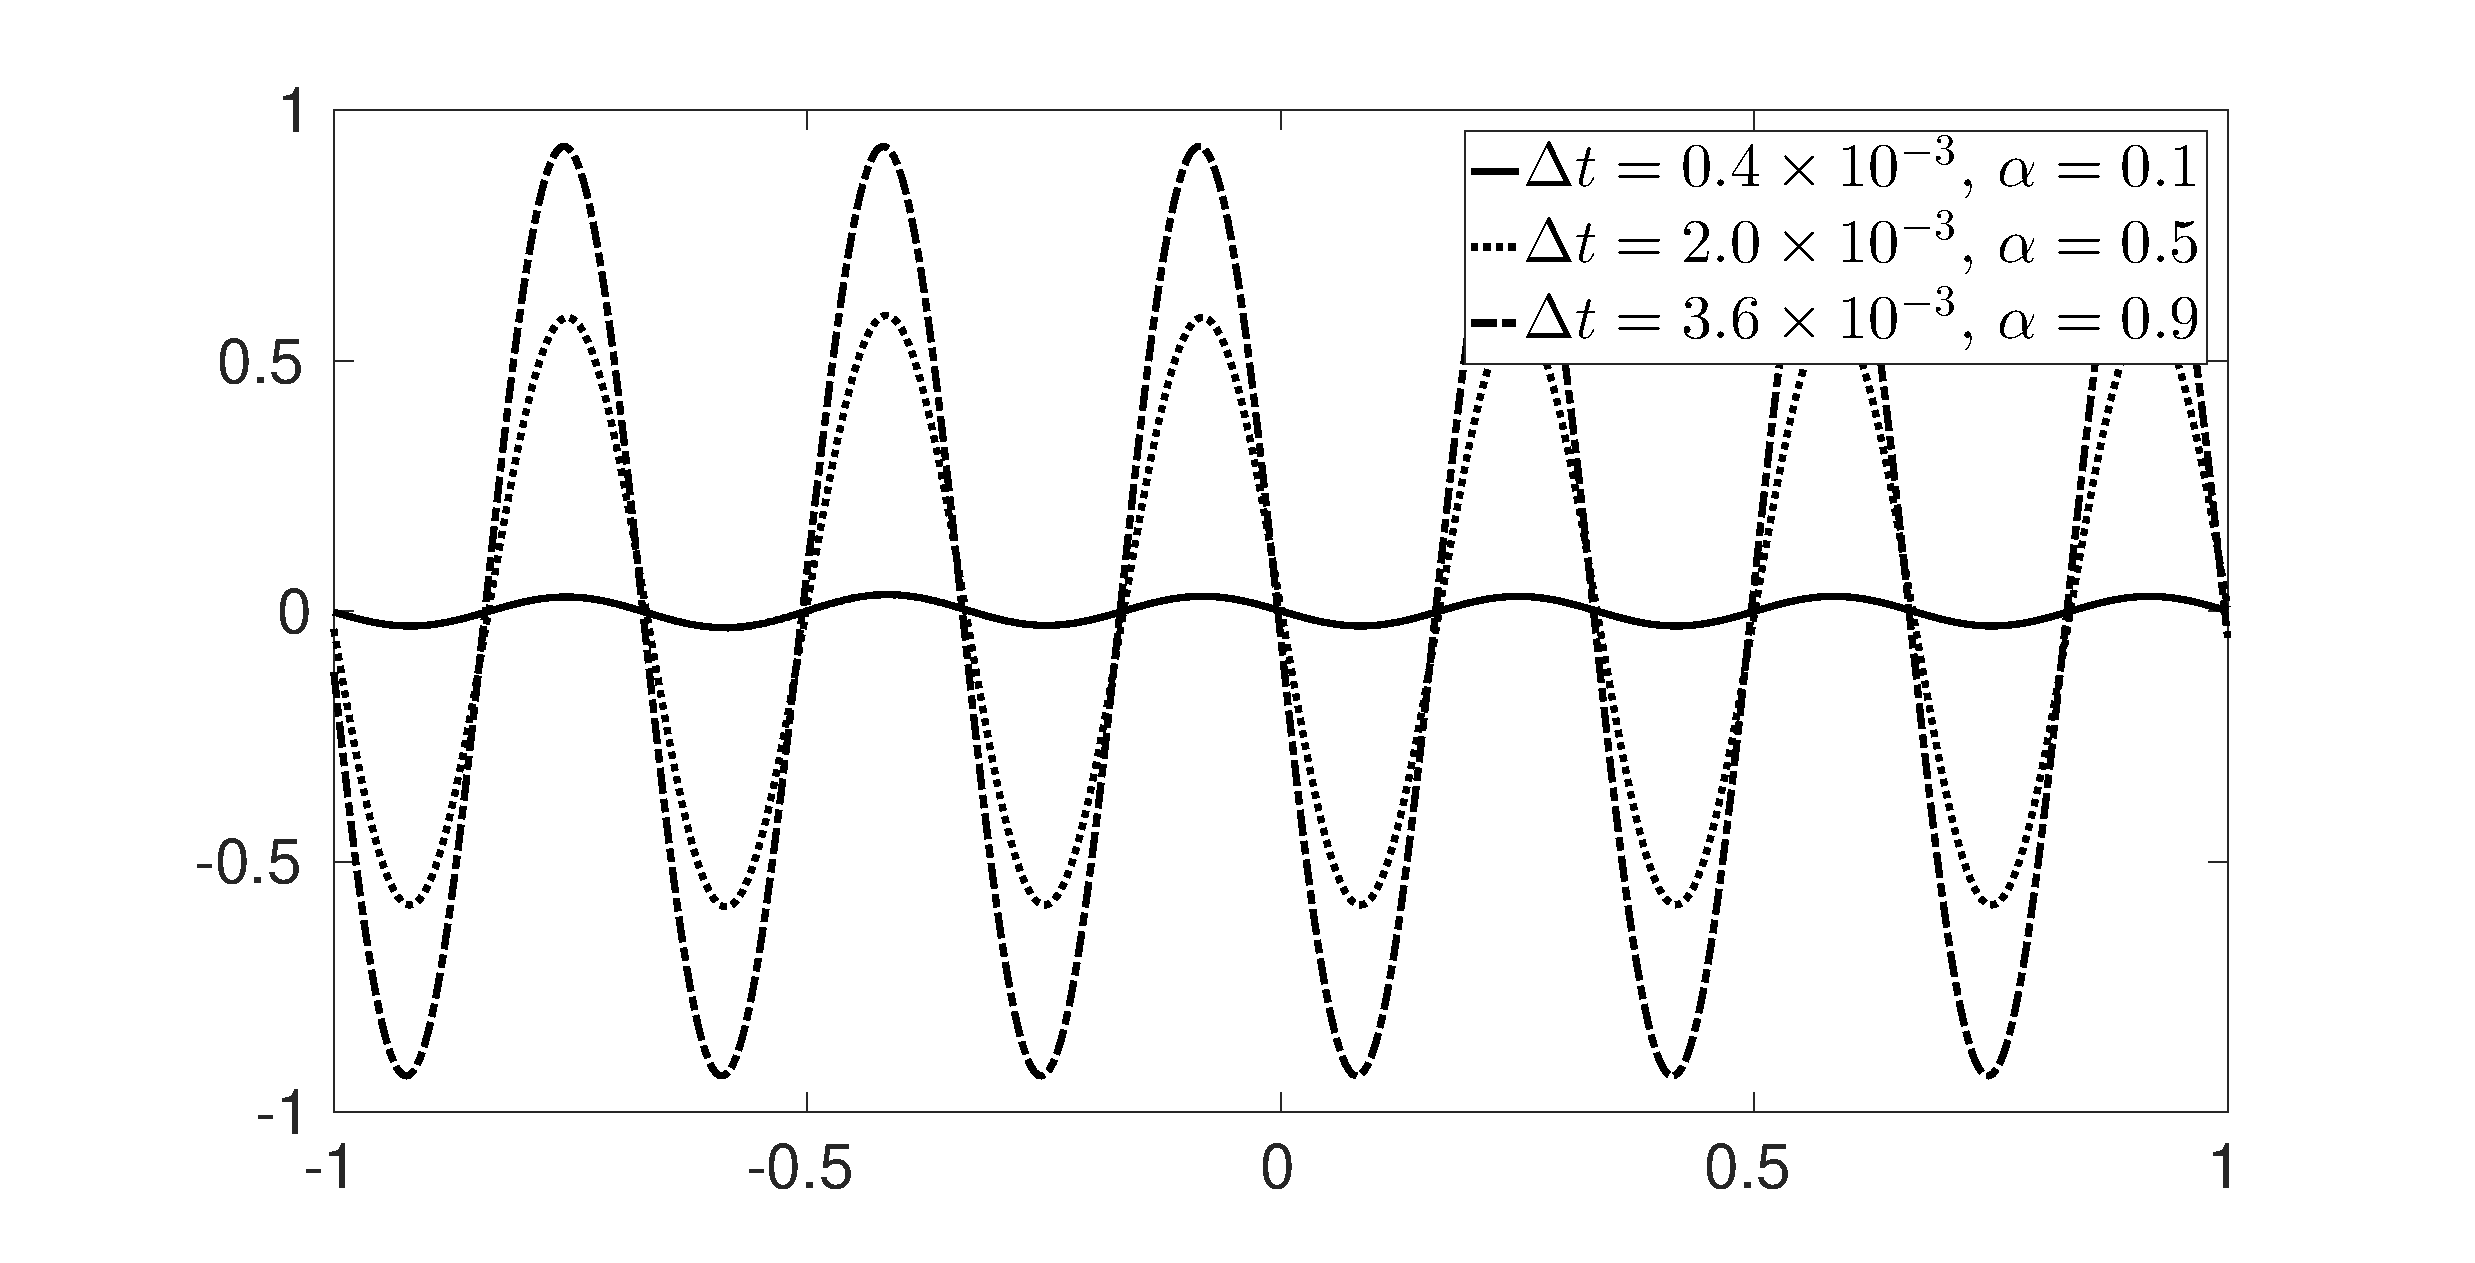
\includegraphics[width=1\textwidth]{1c.eps}
\caption{}
\label{fig:1c}
\end{figure}


\subsection{Numerical dispersion}
\begin{figure}
\centering
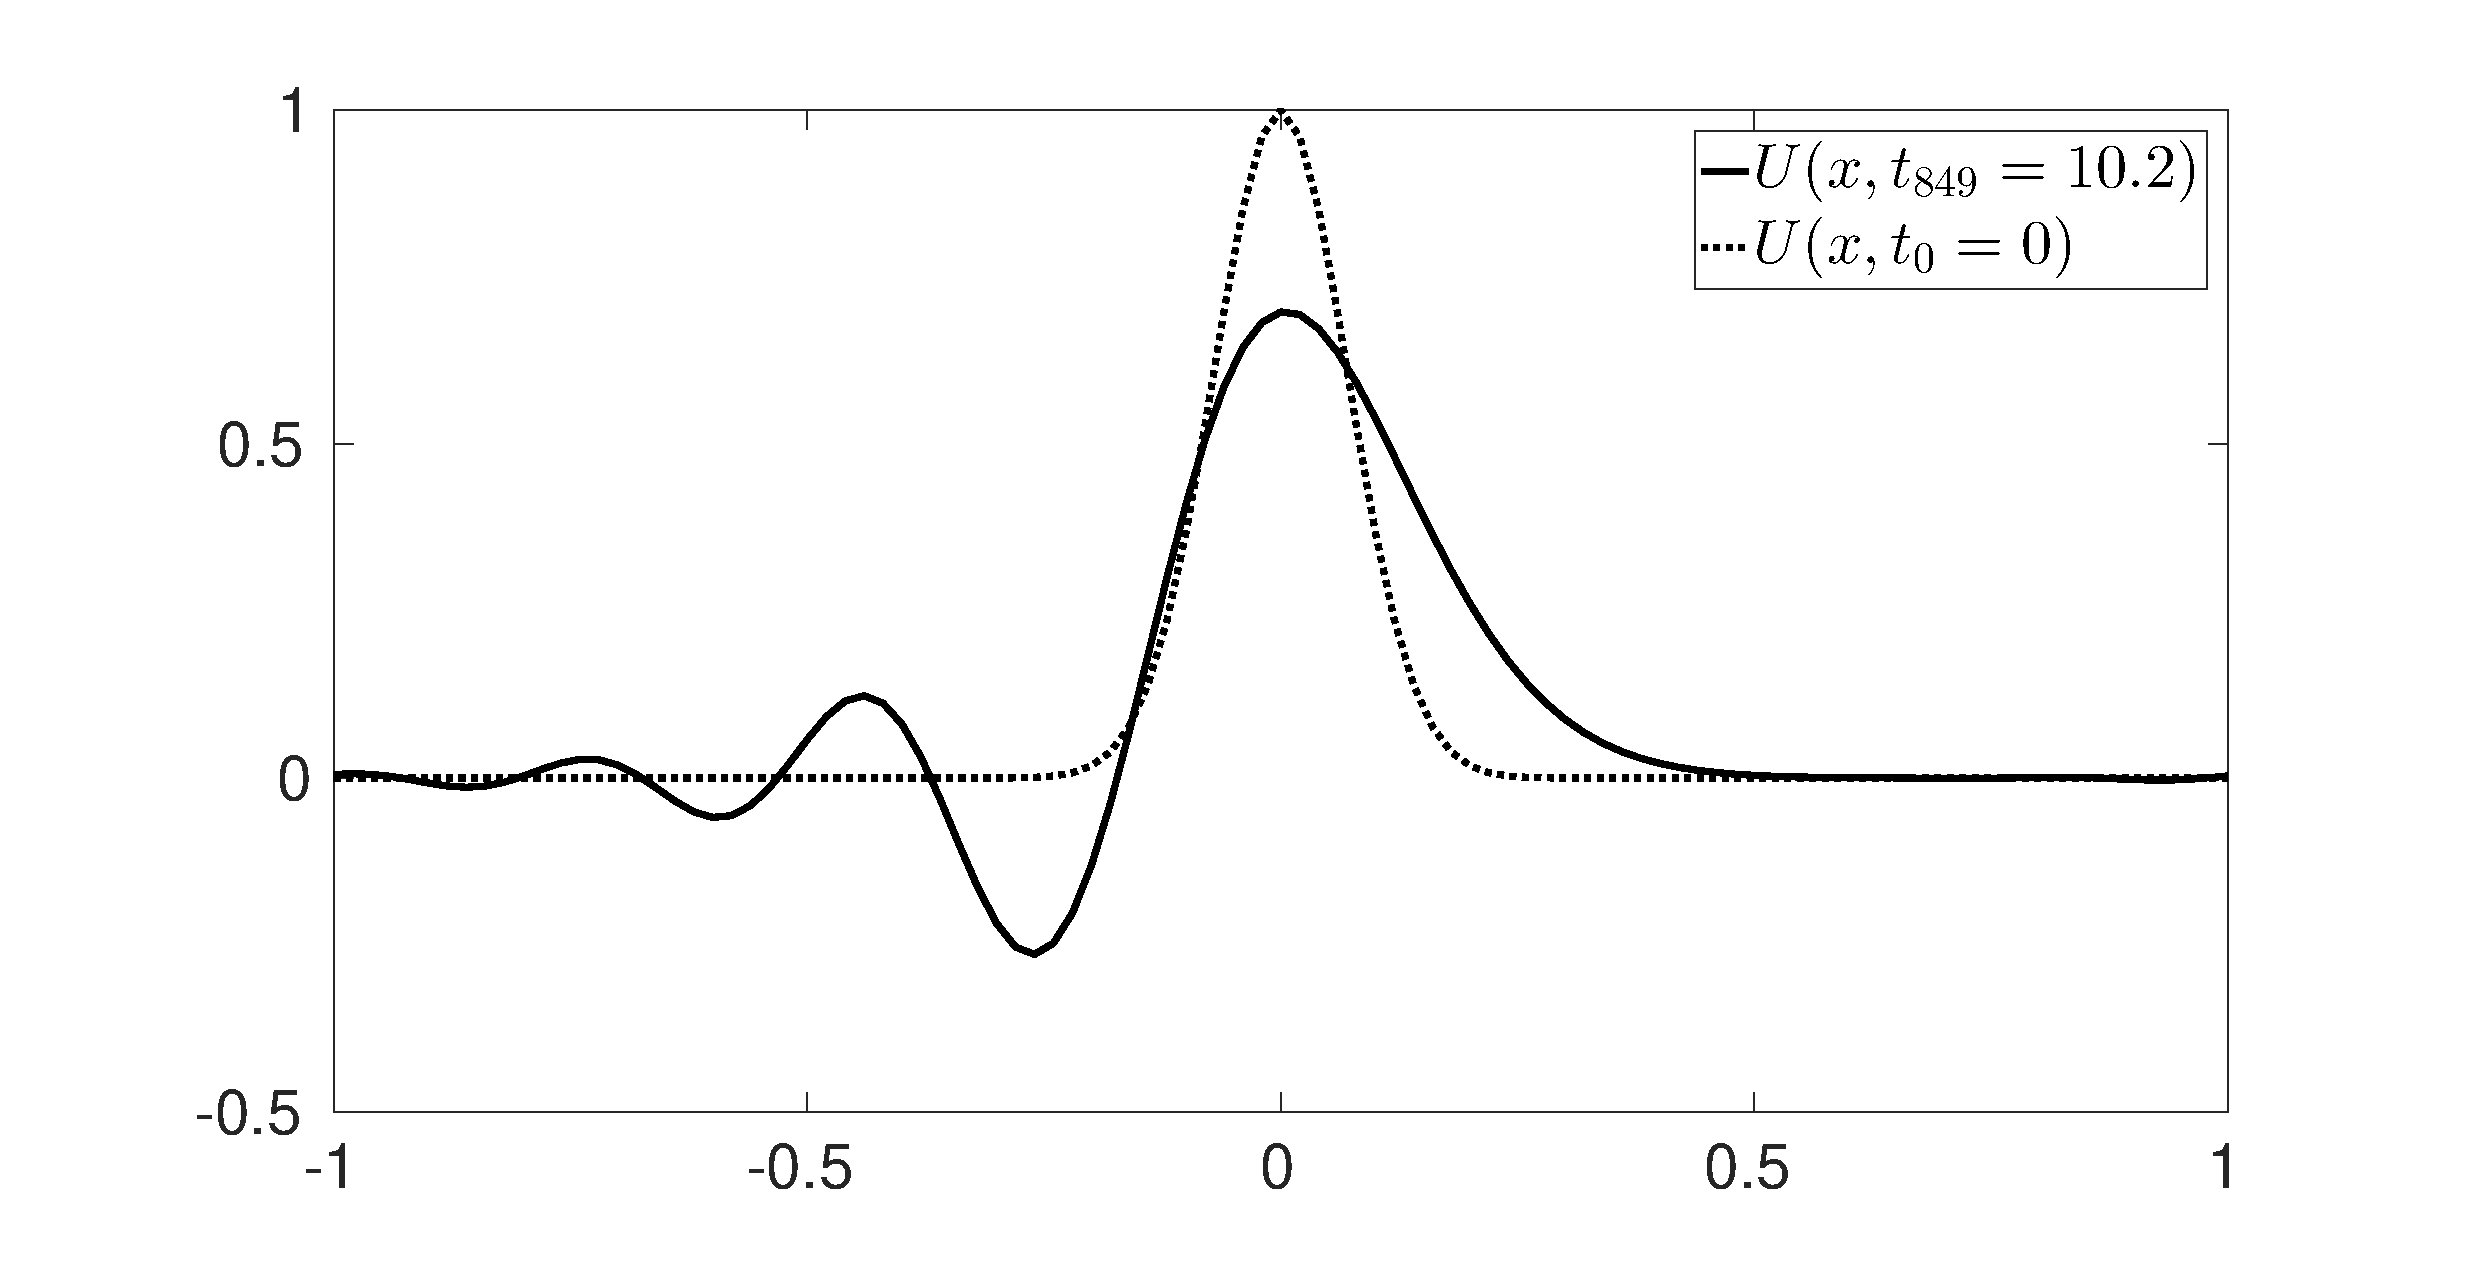
\includegraphics[width=1\textwidth]{1d.eps}
\caption{}
\label{fig:1d}
\end{figure}



\subsection{Other remarks}



\section{Stability of a scheme for the advection equation}







\end{document}




%  LocalWords:  MFT MF Advection PDE's AMATH IC discretization MATLAB
